\documentclass[12pt]{beamer}
\setbeamersize{text margin left=5mm, text margin right=5mm}
\beamertemplatenavigationsymbolsempty
\setbeamertemplate{footline} {
  \leavevmode%
  \hbox{%
    \begin{beamercolorbox}[wd=.35\paperwidth, ht=2.25ex, dp=1ex, left]{section in head/foot}%
      \usebeamerfont{author in head/foot}\hspace*{2.5mm}\insertshortauthor
    \end{beamercolorbox}%
    \begin{beamercolorbox}[wd=.55\paperwidth, ht=2.25ex, dp=1ex, center]{title in head/foot}%
      \usebeamerfont{title in head/foot}\insertshorttitle
    \end{beamercolorbox}%
    \begin{beamercolorbox}[wd=.10\paperwidth, ht=2.25ex, dp=1ex, right]{date in head/foot}%
      \usebeamerfont{date in head/foot}
      \insertframenumber{} / \inserttotalframenumber\hspace*{2.5mm}
    \end{beamercolorbox}%
  }
  \vskip0pt%
}

\usepackage{textcomp}
\usepackage{tikz}
\usepackage{listings}
\lstset{basicstyle=\fontsize{8}{9}\sffamily, columns=flexible, breaklines=true, frame=single}

\title{Deployment of SCION on Bare Metal Switches}
\author{Lars-Christian Schulz \and Cecil Benjamin Leonard}
\date{\today}

\begin{document}

\begin{frame}[plain]
\maketitle
\end{frame}

\section{Introduction}
\begin{frame}
\frametitle{Introduction}
\begin{itemize}
    \item SCION is an internet architecture that is capable of routing control, failure isolation, and explicit trust information for end-to-end communication
    \item Bare-metal switch is a network device without network operating system.We can decide on an operating system.It is cheaper and features based on operating system can be customized when in comparison to a closed switches.
    \item We aim to implement the SCION on an Edgecore Network's bare metal switches
\end{itemize}
\end{frame}

%%%%%%%%%%%%%%%%%%%%%%%%%%%%%%%

\section{Switch Hardware}
\begin{frame}
\frametitle{Outline}
\tableofcontents[currentsection]
\end{frame}

\begin{frame}
\frametitle{Switch Hardware}
\begin{itemize}
    \item SCION is deployed on two Edgecore switches an AS4610-54T and an AS5812-54T.
    \item Switch AS4610-54T utilizes a Broadcom BCM56340 Helix4 switching ASIC and a dual-core ARM Cortex A9 at 1~GHz with 2~GB of DDR3 SDRAM. 
    \item Switch AS5812-54T has a Intel Atom C2538 quad-core 2.4 GHz x86 processor. Broadcom BCM56864 Trident2 switching ASIC.
\end{itemize}
\end{frame}

%%%%%%%%%%%%%%%%%%%%%%%%%%%%%%%

\section{Choosing a NOS}
\begin{frame}
\frametitle{Outline}
\tableofcontents[currentsection]
\end{frame}

\begin{frame}{Choosing a Network Operating System}
\begin{itemize}
    \item SCION can run on multiple platforms such as Ubuntu, ARM mini computers, Android devices.
    \item Network Operating Systems - PICA OS, Cumulus OS. ONL, OpenSwitch (OPX)
    \item We chose Open Network Linux because it is an open source operating system
    \item It is supported and can be implemented on most of the available processors.
    \item We are using Debian9 based armel as the operating system in AS4610-54T
    \item Debian9 AMD64 is used as an operating system in AS5812-54T.
    \end{itemize}
\end{frame}

%%%%%%%%%%%%%%%%%%%%%%%%%%%%%%%

\section{Running SCION on Open Network Linux}
\begin{frame}
\frametitle{Outline}
\tableofcontents[currentsection]
\end{frame}

\begin{frame}
\frametitle{Running SCION on Open Network Linux}
\framesubtitle{ARM}
\begin{itemize}
    \item SCION and its dependencies are compatible with Ubuntu environment and ONL is Debian based operating system.
    \item Installation of SCION in Debian 8 based armhf ONL
    \begin{itemize}
        \item Python has to be upgraded. As the default version is too old. 
        \item Capnproto and libcapnp-dev packages are unavailable in Debian 8 hence installed it from Jessie-backports
    \end{itemize}
    \item Installation of SCION in Debian9 based armhf ONL
    \begin{itemize}
        \item Error when installing cryptography. So upgraded the version of cryptography
        \item Error with ZLOG files.
        \item Setcap command failed because of kernel configuration.
        \item SCION was unable to find if docker is running or not.
    \end{itemize}
\end{itemize}
\end{frame}

\begin{frame}
\frametitle{Running SCION on Open Network Linux}
\framesubtitle{x86}
\begin{itemize}
     \item Installation of SCION in Debian9 based x86 ONL
    \begin{itemize}
        \item Issue with Cryptography installation. Cryptography has a dependence on pyopenssl. When cryptography was upgraded and pyopenssl was also upgraded. Pip3 stopped working so pyopenssl was reinstalled with lower version.
        \item Setcap command failed so installed libcap2-bin.
        \item Bandwidth test and sensor fetch were tested.
        \item SCION is moved to a USB drive because SCION logs files could cause flash memory full in the switch. Better solution would be to use an network file storage system.
    \end{itemize}
\end{itemize}
\end{frame}

\begin{frame}
\frametitle{Running SCION on Open Network Linux}
\framesubtitle{SCION traffic on a physical loop connection}
\begin{itemize}
    \item Map SCION UDP overlay connections to switch ports
\end{itemize}
\center
\scalebox{0.8}{
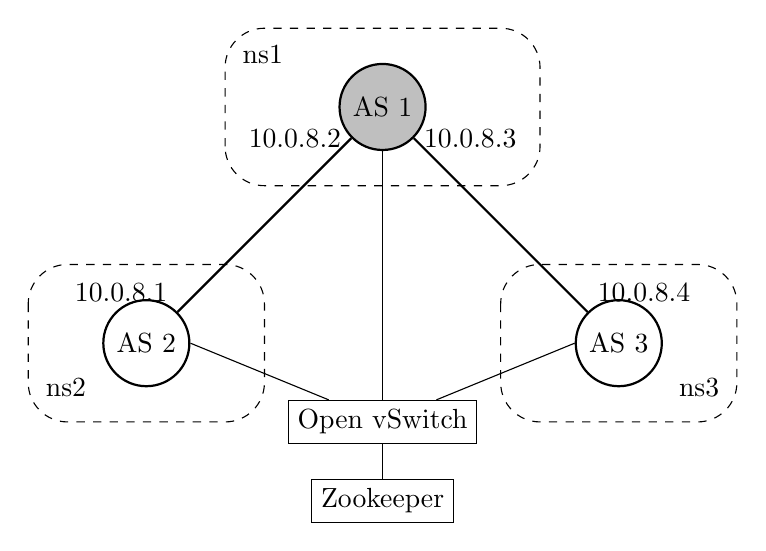
\begin{tikzpicture}
\node at (0, 0) [circle, thick, draw, fill=lightgray] (AS1) {AS 1};
\node at (-3cm, -3cm) [circle, thick, draw] (AS2) {AS 2};
\node at (3cm, -3cm) [circle, thick, draw] (AS3) {AS 3};

\node at (0cm, -4cm) [rectangle, draw] (OVS) {Open vSwitch};
\node at (0cm, -5cm) [rectangle, draw] (zookeeper) {Zookeeper};

\draw[thick] (AS1.south west) node[anchor=east] {10.0.8.2} -- (AS2.north east) node[anchor=south east] {10.0.8.1};
\draw[thick] (AS1.south east) node[anchor=west] {10.0.8.3} -- (AS3.north west) node[anchor=south west] {10.0.8.4};

\draw[thin, dashed, rounded corners=5mm] (-2cm, -1cm) rectangle (2cm, 1cm);
\node at (-1.9cm, 0.9cm) [anchor=north west] {ns1};
\draw[thin, dashed, rounded corners=5mm] (-4.5cm, -2cm) rectangle (-1.5cm, -4cm);
\node at (-4.4cm, -3.8cm) [anchor=south west] {ns2};
\draw[thin, dashed, rounded corners=5mm] (1.5cm, -2cm) rectangle (4.5cm, -4cm);
\node at (4.4cm, -3.8cm) [anchor=south east] {ns3};

\draw[thin] (AS1.south) -- (OVS);
\draw[thin] (AS2.east) -- (OVS);
\draw[thin] (AS3.west) -- (OVS);
\draw[thin] (zookeeper) -- (OVS);
\end{tikzpicture}
}
\begin{itemize}
    \item Isolate ASes in network namespaces to force packets out the physical network interfaces
    \item Open vSwitch connections for infrastructure management
\end{itemize}
\end{frame}

%%%%%%%%%%%%%%%%%%%%%%%%%%%%%%%

\section{Switch Fabric APIs}
\begin{frame}
\frametitle{Outline}
\tableofcontents[currentsection]
\end{frame}

\begin{frame}
\frametitle{Open Switch APIs (Broadcom)}
\begin{itemize}
    \item At this point the switches are just slow general-purpose computers running Linux
    \item Need a way to control and configure the switching chip
    \vspace{5mm}
    \item Public APIs available from Broadcom:
    \begin{itemize}
        \item OpenNSL (Open Network Switch Layer)
        \item OF-DPA (OpenFlow Data Plane Abstraction)
        \item SAI (Switch Abstraction Interface)
        \item SDKLT (Logical Table Software Development Kit)
    \end{itemize}
\end{itemize}
\end{frame}

\begin{frame}
\frametitle{OpenNSL}
\framesubtitle{Overview}
\begin{columns}
\begin{column}{0.5\textwidth}
\begin{itemize}
    \item Abstracts a wide range of Broadcom switch ASICs
    \item General switch operation, configuring and monitoring ports
    \item Warm boot (restart without disrupting the data plane)
    \item Control L2 switching and L3 routing tables
    \item VLANs, QoS, L2 multicast, trunking, tunneling, ...
\end{itemize}
\end{column}
\begin{column}{0.5\textwidth}
\center
\includegraphics[width=0.7\textwidth]{images/opennsl_components.png}\\
\scriptsize Source: OpenNSL White Paper (June 2016)
\end{column}
\end{columns}
\end{frame}

\begin{frame}
\frametitle{OpenNSL}
\framesubtitle{Overview}
\begin{itemize}
    \item Packet Tx/Rx API
    \begin{itemize}
        \item Bypass the Linux network stack \textrightarrow Could improve border router speed
    \end{itemize}
    \pause
    \item Kernel Network (KNET)
    \begin{itemize}
        \item Creates virtual network interfaces connecting switch fabric to the CPU
        \item Switch ports become accessible from Linux
        \item Can match arbitrary packet data \textrightarrow Could match hop fields in the SCION header
    \end{itemize}
    \pause
    \item Field Processor API
    \begin{itemize}
        \item Match header fields, classify packets and take according actions
        \item Might be able to match arbitrary user-defined header fields
    \end{itemize}
\end{itemize}
\end{frame}

\begin{frame}
\frametitle{OpenNSL}
\framesubtitle{Overview}
\begin{itemize}
    \item C interface and usage examples published on GitHub\footnote{\url{https://github.com/Broadcom-Switch/OpenNSL}}
    \begin{itemize}
    	\item ``Community Development Package''
    \end{itemize}
    \item Implementation is closed source and binaries are provided by switch vendors
    \begin{itemize}
    	\item ``OEM/ODM Development Package'' available under a license agreement
    	\item Some platform customization through configuration scripts without recompiling
    \end{itemize}
    \item OpenNSL exposes a subset of the full Broadcom SDK
\end{itemize}
\end{frame}

\begin{frame}[fragile]
\frametitle{OpenNSL}
\framesubtitle{Compiling the Examples}
\begin{itemize}
    \item Binaries supplied by Edgecore
    \item Example source code from GitHub supplied by Broadcom
    \pause
    \item x86-64: compiles and works
    \pause
    \item ARM: missing symbols
\begin{lstlisting}
bin/as4610/libopennsl.so.1: undefined reference to `bcm_ether_atoe'
bin/as4610/libopennsl.so.1: undefined reference to `bcm_ether_ntoa'
\end{lstlisting}
    \item Slight version mismatch between examples source code (3.5.0.1) and OpenNSL binary (3.5.0.3)
    \item bcm\_ether\_atoe and bcm\_ether\_ntoa are utility functions used in some Broadcom code
    \item Can link them in from another source
\end{itemize}
\end{frame}

\begin{frame}
\frametitle{OpenNSL}
\framesubtitle{Compiling the Kernel Modules}
\begin{itemize}
    \item OpenNSL relies on three modules loaded in the Linux kernel: \texttt{linux-kernel-bde}, \texttt{linux-user-bde} and \texttt{linux-bcm-knet}
    \item Edgecore provides OpenNSL only for ONL based on the armel port of Debian
    \item User space library for armel can run on armhf too
    \item Kernel modules do not work with a kernel they have not been compiled for
    \item GPL-licensed kernel module source code is available
\end{itemize}
\end{frame}

\begin{frame}
\frametitle{OpenNSL}
\framesubtitle{Compiling the Kernel Modules}
\begin{itemize}
    \item Makefiles supplied with OpenNSL seem quite outdated
    \item Compiling for an x86-64 architecture and Linux 4.4 (Ubuntu 16.04) worked, but we are running Kernel 4.14 on ARM (armhf)
    \pause
    \item Combined existing makefiles for different kernel versions and architectures
    \item No success yet, because of removed/changed kernel APIs
    \pause
    \item Updated code for Kernel 4.14 \textrightarrow Modules compile successfully
    \pause
    \item Loading the modules still fails, not enough memory for DMA
    \item Lowering amount of memory allocated for DMA from 4~MB to 2~MB works
    \pause
    \item Result: \texttt{linux-kernel-bde} fails to detect the switch hardware
\end{itemize}
\end{frame}

\begin{frame}[fragile]
\frametitle{OpenNSL}
\framesubtitle{Summary}
\begin{itemize}
    \item OpenNSL working on both switches
    \item Can compile examples and our own programs on both switches
    \begin{itemize}
        \item Send and receive packets, configure VLANs, get statistics
        \item Create KNET interfaces and filters
\begin{lstlisting}
>add netif 1 port1
Created interface port1 ID: 1
Created filter port1 ID: 2
>ls netif
ID: 1, Port: 1, VLAN: 0, Name: "port1", MAC: 02:10:18:00:00:01
>ls filter
ID: 2, Priority: 100, Ingress port: 1, DestID: 1, Description: "port1"
ID: 1, Priority: 255, Ingress port: 0, DestID: 0, Description: "DefaultRxAPI"
\end{lstlisting}
        \item Use the field processor to classify packets
\begin{lstlisting}
>ls field_group
Field Group: priority: -2147483647 to 2147483647, entries: 1/16384, counters: 0/16384, meters: 0/16384
\end{lstlisting}
    \end{itemize}
\end{itemize}
\end{frame}

\begin{frame}
\frametitle{OF-DPA}
\begin{columns}
\begin{column}{0.5\textwidth}
\begin{itemize}
    \item C API enabling implementation of OpenFlow 1.3.4
    \item Uses the same software infrastructure as OpenNSL
    \item Reference implementation of an OpenFlow agent and examples on GitHub\footnotemark
\end{itemize}
\end{column}
\begin{column}{0.5\textwidth}
\center
\includegraphics[width=0.9\textwidth]{images/of-dpa_components.png}
\scriptsize Source: OF-DPA: Abstract Switch Specification Version 2.01
\end{column}
\end{columns}
\footnotetext{\url{https://github.com/Broadcom-Switch/of-dpa}}
\end{frame}

\begin{frame}[fragile]
\frametitle{OF-DPA}
\begin{itemize}
    \item Since OpenFlow 1.2: Extensible Match (OXM) format to describe match rules
    \begin{itemize}
        \item Supports ``experimenter'' extensions
        \item OF-DPA specification describes some experimenter header fields
        \item No user-defined header fields
    \end{itemize}
    \pause
    \item Test application to send packets between switches
\begin{lstlisting}
>add flow rx 1
>dump table 60 10
Table  60: ACL Policy
Entries: 1 / 3840
Entry 0:  inPort:mask = 1:0xffffffff srcMac:mask = 0000.0000.0000:0000.0000.0000 destMac:mask = 0000.0000.0000:0000.0000.0000 etherType:mask = 0x0000:0x0000 | GoTo = 0 (None) outPort = CONTROLLER (Reserved)  | priority = 0 hard_time = 0 idle_time = 0 cookie = 0
>rx 1
No more packets available
\end{lstlisting}
\end{itemize}
\end{frame}

\begin{frame}
\frametitle{SAI and SDKLT}
\begin{itemize}
    \item SAI (Switch Abstraction Interface)
    \begin{itemize}
        \item Vendor-independent switch API under the umbrella of the Open Compute Project\footnote{\url{https://github.com/opencomputeproject/SAI}}
        \item Broadcom's implementation\footnote{\url{https://github.com/Broadcom-Switch/SAI}} is a wrapper around OpenNSL
    \end{itemize}
\end{itemize}
\begin{itemize}
    \item SDKLT (Logical Table Software Development Kit)
    \begin{itemize}
        \item Similar aim to OpenNSL
        \item More direct access to forwarding tables
        \item Low-level API is documented
        \item Implementation is open source\footnote{\url{https://github.com/Broadcom-Network-Switching-Software/SDKLT}}
        \item Currently only available for BCM56960 Tomahawk devices
    \end{itemize}
\end{itemize}
\end{frame}

%%%%%%%%%%%%%%%%%%%%%%%%%%%%%%%

\section{Summary and Future Work}

\begin{frame}
\frametitle{Outline}
\tableofcontents[currentsection]
\end{frame}

\begin{frame}
\frametitle{Summary and Future Work}
\begin{itemize}
    \item Selected a suitable OS for the bare-metal switches
    \item Installed SCION on Debian 8 (Jessie), Debian 9 (Stretch)
    \item SCION running on a bare-metal switch
    \item Evaluated switch fabric APIs for use in SCION border router
    \begin{itemize}
        \item OpenNSL might be able to help, but not sure yet
    \end{itemize}
\end{itemize}
\end{frame}

\end{document}
